%%%%%%%%%%%%%%%%%%%%%%%%%%%%%%%%%%%%%%%%%%%%%%%%%%%%%%%%%%%%

\documentclass{article}
\pdfpagewidth=8.5in
\pdfpageheight=11in
\usepackage{ijcai18}

%%%%%%%%%%%%%%%%%%%%%%%%%%%%%%%%%%%%%%%%%%%%%%%%%%%%%%%%%%%%

\newif\ifreview
\reviewtrue
%\reviewfalse

\newif\ifshort
\shorttrue
%\shortfalse

\newif\ifincludeappendices
%\includeappendicestrue
\includeappendicesfalse

\newcommand{\noreview}[1]{\ifreview \else #1 \fi}
\newcommand{\longversion}[1]{\ifshort \else #1 \fi}
\newcommand{\tryinline}[1]{
  \ifshort $\ensuremath{#1}$ 
  \else \[\ensuremath{#1}\] 
  \fi}

%%%%%%%%%%%%%%%%%%%%%%%%%%%%%%%%%%%%%%%%%%%%%%%%%%%%%%%%%%%%

% Use the postscript times font!
\usepackage{times}
\usepackage{xcolor}
\usepackage{soul}
\usepackage[utf8]{inputenc}
\usepackage[small]{caption}

\usepackage[noend]{algorithmic}
\usepackage{algorithm}
\algsetup{linenodelimiter=.\ }
\algsetup{indent=1.5em}
%\algsetup{linenosize=\footnotesize}
\algsetup{linenosize=\scriptsize}


\usepackage{graphicx}
\usepackage{paralist}
\usepackage{flushend}
\usepackage{hyperref}
\usepackage{setspace}
\usepackage{enumitem}
\usepackage{multirow}
\usepackage{rotating}

\usepackage{amsmath}
\usepackage{amssymb}
\usepackage{amsthm}
\newtheorem{theorem}{Theorem}
\newtheorem*{theorem*}{Theorem}
\newtheorem{proposition}{Proposition}
\newtheorem*{proposition*}{Proposition}
\newtheorem{definition}{Definition}
\newtheorem*{definition*}{Definition}

\title{
  \setstretch{1.15}
  Counterfactual Resimulation for Causal Analysis of
  Rule-Based Models
}

\ifreview
\author{Anonymous authors}
%\setlength\titlebox{2in}
\else
\author{
  Jonathan Laurent$^1$,
  Jean Yang$^1$,
  Walter Fontana$^2$, \\
  %
  $^1$ Carnegie Mellon University \\
  $^2$ Harvard Medical School \\
  % 
  \{jonathan.laurent,\ jyang2+\}@cs.cmu.edu, \ 
  % jonathan.laurent@cs.cmu.edu, \ 
  % jyang2+@cs.cmu.edu, \ 
  walter\_fontana@hms.harvard.edu
}
\fi

\ifshort\ifreview
%\setlength\titlebox{2.5in}
\setlength\titlebox{2.0in}
\fi\fi
%%%%%%%%%%%%%%%%%%%%%%%%%%%%%%%%%%%%%%%%%%%%%%%%%%%%%%%%%%%%


%%%%%%%%%%%%%%%%%%%%%%%%%%%%%%%%%%%%%%%%%%%%%%%%%%%%%%%%%%%%
% Formatting macros

%\newcommand{\m}[1]{{\small\textsf{#1}}}
\newcommand{\m}[1]{{\textsc{#1}}}
\newcommand{\TODO}[1]{[\textsl{#1}]}

%%%%%%%%%%%%%%%%%%%%%%%%%%%%%%%%%%%%%%%%%%%%%%%%%%%%%%%%%%%%
% Math Macros

\newcommand{\Nat}{{\mathbb N}}
\newcommand{\Real}{{\mathbb R}}
\newcommand{\eqdef}{\triangleq}

\newcommand{\Prob}[1]{\mathbf{P} \left\{\, #1 \,\right\}}
\newcommand{\ProbParen}[1]{\mathbf{P} \left(\, #1 \,\right)}
\newcommand{\ProbParenSmall}[1]{\mathbf{P}\left(#1\right)}
\newcommand{\CProb}[2]{\Prob{#1 \ |\  #2}}

%%%%%%%%%%%%%%%%%%%%%%%%%%%%%%%%%%%%%%%%%%%%%%%%%%%%%%%%%%%%
% Kappa notations

% Left-hand side and right-hand side of a rule
\newcommand{\RLHS}[1]{L_{#1}}
\newcommand{\RRHS}[1]{R_{#1}}

% State in a trace
%\newcommand{\TSTATE}[2]{\m{State}_{#1}(#2)}
%\newcommand{\TSTATE}[2]{\left[#2\right]^{#1}}
%\newcommand{\TSTATE}[2]{#2^{[#1]}}
%\newcommand{\TSTATE}[2]{#2[#1]}
\newcommand{\TSTATE}[2]{#2\text{\footnotesize$[#1]$}}

% Embeddings and divergent embeddings
\newcommand{\EMBS}[2]{\m{Emb}_{#1}(#2)}
\newcommand{\DEMBS}[2]{\m{Emb}'_{#1}(#2)}
%\newcommand{\EMBS}[2]{\mathcal{E}'_{#1}(#2)}
%\newcommand{\DEMBS}[2]{\mathcal{E}'_{#1}(#2)}

% Executable potential event
\newcommand{\TRIGGERABLE}[2]{#1 \vdash #2}

% Updating a mixture
\newcommand{\UPDATE}[2]{#1\nolinebreak\boldsymbol{\cdot}\nolinebreak#2}
%\newcommand{\UPDATE}[2]{#1 \,!\, #2}

% Time of an event
\newcommand{\TIME}[1]{\textsc{time}(#1)}

%%%%%%%%%%%%%%%%%%%%%%%%%%%%%%%%%%%%%%%%%%%%%%%%%%%%%%%%%%%%
% Macros for counterfactuals

% Altered and counterfactual traces
\newcommand{\ATRAJ}[0]{{T_\iota}}
\newcommand{\CTRAJ}[0]{{T_\iota\,|\,\{T=\tau\}}}

% 'blocked' predicate
\newcommand{\BLOCKED}[2]{\m{blocked}_{#1}[#2]}

% Typical counterfactual statement
\newcommand{\CFST}[0]{\tau \models [\iota] \, \psi}

% Reference trace
%\newcommand{\RefTrace}{trace~(\ref{example-trace})}
%\newcommand{\RefTrace}{trace~\ref{example-trace}}
\newcommand{\RefTrace}{trace~{\small(\ref{example-trace})}}

\begin{document}

\maketitle

% -*- TeX-master: "ijcai18.tex" -*-

\begin{abstract}
  Models based on rules that express local and heterogeneous mechanisms
  of stochastic interactions between structured agents are an
  important tool for investigating the dynamical behavior of complex
  systems, especially in molecular biology. Given a simulated trace of
  events, the challenge is to construct a causal diagram that explains
  how a phenomenon of interest occurred. Counterfactual analysis can
  provide distinctive insights, but its standard definition is not
  applicable in rule-based models because they are not readily
  expressible in terms of structural equations. We provide a semantics
  of counterfactual statements that addresses this challenge by
  sampling counterfactual trajectories that are probabilistically as
  close to the factual trace as a given intervention permits them to
  be. We then show how counterfactual dependencies give rise to
  explanations in terms of relations of enablement and prevention
  between events.
\end{abstract}
% -*- TeX-master: "ijcai18.tex" -*-

\section{Introduction}\label{sec:intro}

Rule-based modeling languages for molecular biology, such as Kappa
\cite{DanosEtAl-CONCUR07} and BioNetGen \cite{bngl}, or organic
chemistry, such as M{\o}d \cite{moll}, can be used to write
mechanistic models of complex reaction systems. These approaches
consider entities that have a structure, and make a distinction
between the transformation of a structure fragment (a pattern)
specified by a rule and the reaction resulting from the application
of the rule to a combination of entities contextualizing the
fragment. The structure of bio-molecular entities is conveniently
represented as a graph and a rule is a graph-rewrite directive with a
rate constant that determines its propensity to apply. The stochastic
simulation of a rule collection generates a time series of rule
applications---henceforth events---that might reach a state of
interest in processes like the assembly of a molecular machine, the
activation of a transcription factor, or the synthesis of a specific
compound.

While rule-based models provide compactness, transparency, and the ability of
handling combinatorial complexity, the perhaps most significant advantage lies
in their suitability for causal analysis. This is because such analysis proceeds
at the level of rules, not reactions, thereby avoiding contamination with
context that defines a reaction yet is accidental, because irrelevant, to the
application of the underlying rule. Due to the concurrent nature of events it is
typically far from obvious how a sequence attained a particular
outcome. Biologists often refer to a causal account or explanation as a
``pathway", but have no formal framing for it.

The approach to causal analysis provided in
\cite{DBLP:conf/fsttcs/DanosFFHH12,DanosEtAl-CONCUR07} takes advantage
of rule structure to
\begin{inparaenum}[(i)]
\item \label{step:compress} compress a simulation trace into a minimal
  subset of events that are necessary and jointly sufficient to
  replicate the outcome of interest and
\item \label{step:highlight} highlight causal influences between
  events, exposing the extent of concurrency.
\end{inparaenum}
Such analysis is usually performed on a large sample of traces to the
outcome, thus recovering the salient pathways as those that are
statistically favored by the dynamics. This approach, however, suffers
from two drawbacks. First, the focus on necessity in step
(\ref{step:compress}) neglects events that are kinetically critical
(in that they dramatically increase the probability of observing the
outcome), yet are not logically necessary for achieving it. Second,
step (\ref{step:highlight}) is limited to a narrow notion of causal
influence that we may call \emph{enablement}. Put simply, an event $a$
is said to enable event $b$, if $a$ modifies an aspect of the state of
the world in such a way as to directly permit $b$ to happen. This
positively tinted version of influence is blind to the ubiquitous role
of inhibitory interactions in molecular biology.  Indeed, an event $a$
may cause an event $b$ without (transitively) enabling it, but instead
by preventing another event $c$ that would have prevented
$b$. Clearly, uncovering such an explanatory narrative is challenging
because it involves an event, $c$ in this case, that did \emph{not}
occur in a simulation trace.

We here propose an approach based on counterfactual reasoning that
complements the existing causal analysis of event series generated
from rule-based models. In the tradition of Lewis, Pearl and Halpern,
we investigate possible causal influences by answering questions of
the kind: \textit{Had event $e_1$ not occurred, would event $e_2$ have
  happened?}
% \cite{lewis1974causation,pearl2009causality,halpern2016actual},
Our contributions are as follows.
%\ifshort \begin{inparaenum}[(1)] \else \begin{enumerate} \fi
\begin{enumerate}[leftmargin=0.6cm]
\item We provide a semantics for counterfactual statements in the context of
rule-based models, where the standard definition of counterfactuals based on
structural equations \cite{pearl2009causality,halpern2016actual} does not apply.
\item We show how such statements can be evaluated by sampling
\emph{counterfactual traces} that are meant to probabilistically ``hug" a given
(factual) trace as much as an external intervention permits them to. To this
end, we introduce an algorithm to generate counterfactual traces and provide an
efficient implementation for the Kappa language.
\item We show how counterfactual dependencies between events can be
systematically explained in terms of enablement and prevention relations that
are more in line with biological reasoning.
\end{enumerate}
%\ifshort \end{inparaenum} \else \end{enumerate} \fi

% -*- TeX-master: "ijcai18.tex" -*-

\section{Motivating example}\label{sec:example}

We provide some background on Kappa and introduce a toy
example motivating the need for counterfactual reasoning in analyzing
the causal structure of simulation traces.

\subsection{Some Background on Kappa}\label{sec:background}

Proteins are complex molecular machines that reversibly tag one
another with molecular flags and reversibly bind each other to form
transient associations.  In this way, proteins come to have ``state"
that can control the interactions they engage in. In Kappa, a protein
is modeled as an abstract \emph{agent} with a name that designates its
\emph{type} and a signature of distinguishable \emph{sites} at which
it can be tagged or bound by other agents. A site can bind at most one
agent at a time and must be in a definite state.
% , each type of agent being described in the model's
% \emph{signature}.

In our illustrative example, we consider two types of agents for which
we use biological nomenclature. One type, $S$, is a substrate that
receives a tag known as a phosphate group in a phosphorylation
interaction. The other, $K$, is a kinase that phosphorylates
$S$. Agents of both types feature a binding site at which they can
bind one another and a site that can be in one of two possible states:
\emph{unphosphorylated} or \emph{phosphorylated}. Thus, agents of type
$K$ also have a phosphorylation state, but for the sake of simplicity
we will have them acquire it ``spontaneously".

A \emph{mixture} is a multiset of agents whose state at each site is
fully specified. A mixture represents the state of a system and can be
thought of as a (potentially large) graph consisting of many connected
components. In a mixture, agents of the same type are distinguished by
a unique global identifier. %(Figure~\ref{fig:mixture}).

\begin{figure}[!h]
  \vskip -0.25cm
  \begin{center}
    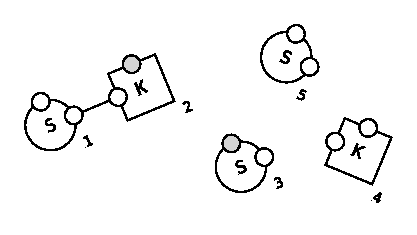
\includegraphics[scale=0.9]{figures/mixture.pdf}
  \end{center}
  \vskip -0.5cm
  \caption{An example of a reaction mixture. Instead of naming sites,
    we here identify them by their position on agents (phosphorylation
    sites are always shown on top). The relative position of agents in
    the figure is insignificant.  Phosphorylated sites are shown in
    gray.  Number labels correspond to global agent identifiers. }
  \label{fig:mixture}
\end{figure}


Interactions between agents are modeled by local rewriting
\emph{rules}.  A rule $r$ is defined by a triple
$(\RLHS{r}, \RRHS{r}, \lambda_r)$, where $\RLHS{r}$ is the left-hand
side specifying a pattern (the pre-condition), $\RRHS{r}$ the
right-hand side (or post-condition), and $\lambda_r$ a firing rate.
The basic idea is that the ``location" at which the mixture matches
$\RLHS{r}$ is rewritten in place by $\RRHS{r}$, changing the state of
the system. (Technically, a rule also requires a function from agents
in $\RLHS{r}$ to agents in $\RRHS{r}$ to make the rewrite
unambiguous.)

% -*- TeX-master: "ijcai18.tex" -*-

\begin{figure}[h]
  \vskip -0.2cm
  \begin{center}
    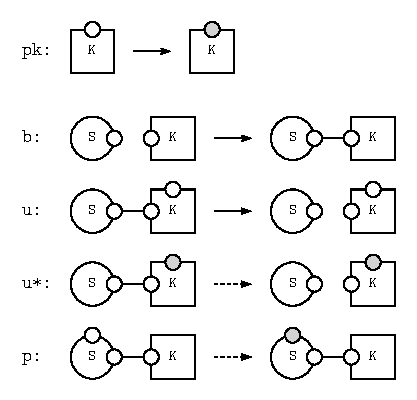
\includegraphics[scale=0.9]{figures/model.pdf}
  \end{center}
  \vskip -0.2cm
  % \caption{A motivating toy model. As usual in Kappa, sites not
  %   mentioned in a rule are left unchanged by it. Instead of naming
  %   sites, we here identify them by their position on an
  %   agent. Phosphorylated sites are shown in gray. Firing rates are
  %   not specified here but dotted arrows indicate \textit{slow}
  %   reactions, whereas solid arrows indicate \textit{fast} reactions.}
  \caption{A motivating toy model. Sites not mentioned in a rule are
    left unchanged by it. \longversion{As in
      Figure~\protect\ref{fig:mixture}, sites are identified by their
      position on an agent.}  Firing rates are not specified, but
    dotted (solid) arrows indicate \textit{slow} (\textit{fast})
    reactions
    $(\lambda_u \gg \lambda_{u^*} \approx \lambda_p)$.}
  \label{fig:model}
\end{figure}


In our toy model, agents are subject to the rules depicted in
Figure~\ref{fig:model}. Rule $b$ states that kinases and substrates
can bind, provided their requisite binding sites are free
(unbound). Note that $\RLHS{b}$ is a pattern: It omits mentioning the
sites that carry phosphorylation state, which are therefore not
considered when matching the mixture to $\RLHS{b}$. Rules $u$ and
$u^{*}$ define unbinding events that depend on the phosphorylation
state of the kinase $K$. The distinction is motivated by kinetics:
Rule $u$ fires at a much faster rate than $u^{*}$. Rule $p$ specifies
that a substrate can be phosphorylated when it is bound to a
kinase. For the sake of simplicity, we model the phosphorylation of a
kinase as a spontaneous process (rule $pk$).

By virtue of the $\lambda_r$, the rules of a model, together with an
initial mixture, constitute a dynamical system that we describe
shortly. We do so in a slightly nonstandard way by introducing the
auxiliary concept of an \emph{event template}. This is to prepare for
the insight in section~\ref{subsec:counterfactuals-semantics} that the
stochastic and deterministic aspects of a model's dynamics can be
cleanly separated, thus enabling counterfactual analysis.

An event template is a pair $(r, \xi)$ where $r$ is a rule and $\xi$ a
function from agents in $\RLHS{r}$ to global identifiers. We say that
$(r, \xi)$ is \emph{realizable} in mixture $m$ if the global
identifiers assigned by $\xi$ exist in $m$ and the agents bearing them
match $\RLHS{r}$. In this case, we write $\TRIGGERABLE{m}{(r, \xi)}$
(read ``$m$ admits $(r, \xi)$") and call $\xi$ an \emph{embedding} of
$\RLHS{r}$ into $m$:
\tryinline{\EMBS{r}{m} \eqdef \{ \xi \,:\,
  \TRIGGERABLE{m}{(r, \xi)}\}.}  Whenever $m \vdash (r, \xi)$, we
write $\UPDATE{m}{(r, \xi)}$ the mixture obtained by
realizing $(r, \xi)$, i.e.\@ by rewriting the agents with identifiers
in the codomain of $\xi$ into $\RRHS{r}$. The realization of an event
template at a particular time creates an (actual) \emph{event},
formally defined as a pair $(e, t)$ with $e$ an event template and $t$
its time of realization.

A model induces a continuous-time Markov chain (CTMC) over the
set of reachable mixtures, where state $m$ transitions to state
$\UPDATE{m}{(r, \xi)}$ at rate $\lambda_r$ for every event template
$(r, \xi)$ that is realizable in $m$. The rate of leaving state $m$ by
an application of rule $r$ is called the \emph{activity} $\alpha_r(m)$
of rule $r$ in
% \ifshort $m$: \else
mixture $m$ and is equal to the product of the rule's firing rate by
the number of embeddings of $\RLHS{r}$ into $m$:
% \fi
$\alpha_r(m)=\lambda_r|\EMBS{r}{m}|$. For example, in
Figure~\ref{fig:mixture}, rule $b$ has activity $2\lambda_b$ and rule
$u$ has activity $0$. The \emph{total activity} of a mixture is defined
as $\alpha(m)=\sum_r\alpha_r(m)=\sum_r\lambda_r|\EMBS{r}{m}|$.
% In terms of CTMC, it corresponds to the total transition rate of $m$.

The CTMC induced by a model can be simulated
with the \emph{Doob-Gillespie algorithm} \cite{gillespie1977exact},
which loops over the following steps:
\begin{inparaenum}[(1)]
\item draw a time interval $\delta$ to the next event from an
  exponential distribution with parameter $\alpha(m)$ and increment
  the simulated system time by $\delta$,
\item draw a rule $r$ with probability $\alpha_r(m)/\alpha(m)$ and
\item pick uniformly an embedding $\xi \in \EMBS{r}{m}$ of $L_r$ into
  $m$ and realize the event template $(r, \xi)$.
\end{inparaenum}
This algorithm is efficiently implemented for rule-based models in
Kappa as described in
\cite{DanosEtAl-APLAS07,BoutillierEK17}\longversion{; it is available
  at kappalanguage.org}. It outputs a sequence of events,
called a \emph{trace}.


\longversion{\begin{algorithm}
\caption{Doob-Gillespie algorithm}\label{alg:gillespie}
\begin{spacing}{1.2}
\begin{algorithmic}
\vspace{0.2cm}
  \STATE $t \gets 0$
  \STATE $m \gets\ $ initial mixture
  \vspace{0.1cm}
  \WHILE{ $t < t_\text{\,end}$ }
      \vspace{0.1cm}
      \STATE $\alpha \gets \sum_r {\lambda_r |\EMBS{r}{m}|}$
      \vspace{0.1cm}
      \STATE draw $\delta \sim \textsc{Exp}(\alpha) $
      \STATE $t \gets t + \delta$
      \STATE draw a rule $r$ with probability
      $\propto \ \lambda_r |\EMBS{r}{m}|$
      \STATE draw an embedding $\xi$ uniformly in $\EMBS{r}{m}$
      %\STATE update $m$ by triggering event $((r, \xi), t)$
      \STATE $m \gets \UPDATE{m}{(r, \xi)}$
      \STATE log event $((r, \xi), t)$
  \ENDWHILE
\vspace{0.1cm}
\end{algorithmic}
\end{spacing}
\end{algorithm}}

\subsection{Where Existing Analysis Falls Short}
\label{subsec:dumb-story}

% What about asking the question for the specific trace to make it
% clearer we are talking about actual causality ?

Consider our toy model and assume, for the sake of illustration, an
initial mixture $I$ with only a single kinase and a single substrate
whose sites are unbound and unphosphorylated. We then ask: Starting
from $I$, \emph{how} is $p$ typically achieved? We are not merely
looking for an account of reachability but for a causal explanation,
i.e.\@ a collection of events connected by causal influences.

For example, a simulation might produce the following trace (events
are labelled by the rules that induced them):
\begin{align}
  \label{example-trace} 
  b,\ \ u,\ \ pk,\ \ b,\ \ p,\ \ u^{*},\ \ \cdots
\end{align} 
Current techniques
\cite{DBLP:conf/fsttcs/DanosFFHH12,DanosEtAl-CONCUR07} generate a
causal account by first computing a \emph{sub-trace} of
(\ref{example-trace}) that is
\begin{inparaenum}[(i)]
\item \emph{valid} in the sense that each of its events can be
  triggered in turn starting from the initial mixture and
\item \emph{minimal} in the sense that none of its valid sub-traces
  features $p$.
\end{inparaenum}
The relations of enablement among events in the minimal sub-trace
yield a directed acyclic graph. Although trivial in our toy example,
minimization is an NP-hard problem. Carrying out this approach on
(\ref{example-trace}), one notes that the first occurence of $b$ sets
the necessary conditions for $p$, but these are subsequently undone by
$u$ only for the second occurrence of $b$ to re-introduce them. This
illustrates why minimization compresses a trace into events that are
\emph{necessary} for the outcome---which requires eliminating futile
cycles. In our case, the causal account for $p$ starts with the
initial condition, symbolized by the \emph{init} event, and skips to
the last $b$ before the $u$. Figure~\ref{fig:dumb-story} depicts the
resulting explanation graph, whose arrows denote enablement as defined
informally in section~\ref{sec:intro} and formally in
section~\ref{sec:inhibition}.

\begin{figure}[H]
  \vskip -0.8cm
  \begin{center}
    \includegraphics[scale=0.7]{figures/dot/dumb-story.pdf}
  \end{center}
  \vskip -1cm
  \caption{A causal explanation for $p$ in trace
    (\ref{example-trace}).  Events are labelled by the rules that
    induced them. The \emph{init} node corresponds to a special event
    that sets the mixture to its initial state.  }
  \label{fig:dumb-story}
\end{figure}


The problem is that the explanation depicted in
Figure~\ref{fig:dumb-story} fails to recognize the critical role of
$pk$ in the original trace. Given the rules of the model, one notes
that $p$ is slow and the average time that $K$ remains bound to $S$
depends on the phosphorylation state of $K$. The kinase $K$ is
phosphorylated in event $pk$, causing the complex between $K$ and $S$
to be sticky, giving the slow phosphorylation $p$ a chance to
occur. It seems reasonable to assert that $p$ would probably not have
happened had $pk$ not happened, since the opportunity for $p$ would
have been curtailed by a fast unbinding event. Thus, $pk$ should be
part of the explanation, although it neither enables $b$ nor $p$
directly (both rules are independent of $K$'s phosphorylation
state). Reasoning of this kind is \emph{counterfactual}
\cite{lewis1974causation,pearl2009causality}.

In section~\ref{sec:counterfactual}, we give a rigorous semantics to
this line of reasoning and introduce an algorithm for simulating
counterfactual scenarios. In section~\ref{sec:inhibition}, we show how
counterfactual dependencies between events can be systematically
explained in terms of a combination of enablement and prevention
arrows, leading to the explanation shown in Figure~\ref{fig:cex}. 
%for the counterfactual dependency between $p$ and $pk$ in our example.

% -*- TeX-master: "ijcai18.tex" -*-

\newcommand{\PCFST}[0]{\ProbParen{\CFST{}}}

\newcommand{\ItAbduction}[0]{(\textit{abduction})}
\newcommand{\ItAction}[0]{(\textit{action})}
\newcommand{\ItPrediction}[0]{(\textit{prediction})}


\section{Evaluating counterfactual
  statements}\label{sec:counterfactual}

In the context of our toy model, the counterfactual statement we must
assess is: ``If $pk$ had not happened, $p$ would not have happened."
Our account in the previous section suggests that $pk$ played a role,
but it is also clear that given the stochastic nature of rule firing
$p$ could well have happened even in the absence of $pk$; it just is
unlikely. In a stochastic setting, counterfactual statements are not
either true or false, but have degrees of likelihood. To assess that
likelihood is our task.

Given an original (factual) trace $\tau$, a naive approach might be to
sample counterfactual traces, each of which starts with the state of
the system attained in $\tau$ just before event $pk$ happened, but in
which we skip over $pk$ and then run an unconstrained simulation from
that point onward. In this approach traces would quickly diverge from
the original, distorting the causal role that $pk$ played specifically
in it. The question here is not what causal role $pk$ can play in
principle, but what role it actually did play in $\tau$. In this
sense, counterfactual statements are undetachable from the context in
which they are formulated.

Pearl's standard account of counterfactual statements
\cite{pearl2009causality} is based on performing \textit{``surgical
  interventions''} on a structural equation model (SEM). A SEM
features a finite sequence $(x_1, \dots, x_n)$ of variables, each
associated to a \emph{functional equation} of the form
$x_i = f_i(x_1, \dots, x_{i-1}, u_i)$, where $f_i$ is a deterministic
function and $u_i$ is a random variable. Ideally, each $f_i$ defines
an independent and autonomous physical mechanism. This is partially
enforced by the requirement that the $u_i$ must be mutually
independent. Given some observation $e$, the probability of the
counterfactual statement ``had $x_j$ been equal to $a$, $\psi$ would
have been be true'' is evaluated following a three-steps process:
\begin{inparaenum}[]
\item \ItAbduction{} compute the distribution $p_e$ of values for
  $\vec u$ given observation $e$, then
\item \ItAction{} intervene in the model by replacing the defining
  equation for $x_j$ by ``$x_j = a$'' and finally
\item \ItPrediction{} compute the probability that $\psi$ is true in
  this new model when $\vec{u}$ is distributed according to $p_e$.
\end{inparaenum}

Because traces generated from rule-based models do not have a natural
encoding in terms of structural equations, Pearl's construction does
not apply straightforwardly in our case.

\subsection{A semantics for counterfactuals}
\label{subsec:counterfactuals-semantics}

An intervention $\iota$ prevents the occurrence of selected events. It
is defined by a predicate $\BLOCKED{\iota}{\cdot}$ ranging over
events. \longversion{(Our framework can accomodate a much broader range of
interventions, but we make this restriction for ease of exposition.)}
Given a predicate $\psi$ over traces, we write the statement
\textit{``Had intervention $\iota$ happened in trace $\tau$, $\psi$
  would have been true''} as $\CFST{}$.

To assign a probability to this statement, it is useful to
reconceptualize the CTMC induced by a model in such a way that the
source of randomness is factored out from the system's state. This can
be done as follows:
\begin{inparaenum}[(i)]
\item Consider all possible potential events $(r, \xi)$, where $\xi$
  maps into a large enough set of global identifiers. If no rule
  creates a new agent, as we shall assume for the sake of simplicity,
  those global identifiers are given by the initial mixture. For each
  one of these potential events, imagine a bell that rings
 according to a Poisson process of parameter
  $\lambda_r$, i.e.\@ the time intervals between consecutive
  ringings are drawn independently from an exponential distribution with
  parameter $\lambda_r$. These Poisson processes are all gathered in
  a random variable $\Sigma$ that we call \emph{schedule}. It features
  the sequence of ring times for every bell and plays the same role as
  the variable $\vec{u}$ in a SEM.
\item A simulation trace can be viewed as a deterministic
  function of $\Sigma$: starting with the initial mixture and
  moving through time, whenever a bell rings, its associated potential
  event $e$ transforms the current mixture $m$ if
  $\TRIGGERABLE{m}{e}$. For example, if the current mixture $m$ is given as in 
  Figure~\ref{fig:mixture} and the bell labeled
  \textit{``apply rule $b$ on substrate $3$ and kinase $4$''} rings, then a bond is created
  between these two agents. However, the bell labeled
  \textit{``apply rule $b$ on substrate $1$ and kinase $2$'}' would have no effect 
  on $m$. We write $T(\sigma)$ the
  particular trace generated from schedule $\sigma$ and
  $T = T(\Sigma)$.
\end{inparaenum}

We extend this viewpoint to include interventions. For an
intervention $\iota$, we define the altered trace $\ATRAJ{}$ much in
the same way as $T$, except that each time the bell associated to $e$
rings at time $t$, we also require $\BLOCKED{\iota}{(e, t)}$ to be
false for $e$ to be executed.  Given an observed trace $\tau$, an
intervention $\iota$ and a predicate $\psi$,
the probability of $\CFST{}$ can now be computed according to Pearl's
three-steps strategy: \ItAbduction{} condition the distribution of
$\Sigma$ by the observation that $T=\tau$, then \ItAction{} alter
the behavior of the simulation with intervention $\iota$ and
\ItPrediction{} compute the probability of $\psi$ in the resulting
setting. This results in the following definition.

\begin{definition}[Semantics of counterfactual statements]\label{def:counterfactuals}
  For $\tau$ an observed trace, $\iota$ an intervention and $\psi$ a
  predicate on traces, the probability of the counterfactual statement
  \textit{``had intervention $\iota$ happened in trace $\tau$,
    predicate $\psi$ would have been true''} is defined as:
  \[ \PCFST{} \eqdef \ \ProbParen{\psi(\ATRAJ{}) \ |\ T = \tau}. \]
\end{definition}

\subsection{The counterfactual resimulation algorithm}
\label{subsec:cosim-algo}

Following Definition~\ref{def:counterfactuals}, we estimate the
probability of the counterfactual statement
$\CFST{}$ by sampling instances of the random
variable $\CTRAJ{}$. Such instances are \emph{counterfactual
  traces}. Intuitively, they give an account of what else trace $\tau$
could have been had intervention $\iota$ happened.  We introduce
Algorithm~\ref{alg:cosimulation}, a variation of the Doob-Gillespie
algorithm, to sample a counterfactual trace efficiently given a
reference trace $\tau$ and an intervention $\iota$. We call it
\emph{counterfactual resimulation}, since it works by going
through every event of $\tau$, resimulating only those parts of $\tau$
that are affected by $\iota$. In particular, when $\iota$ is
the trivial intervention ($\BLOCKED{\iota}{\cdot} = \text{false}$), it
returns $\tau$.

This algorithm relies on a modified notion of activity we call
\emph{divergent activity}. We define the set of \emph{divergent
  embeddings} of the left-hand side of a rule $r$ into mixture $m$
and relative to $m_0$ as
%\tryinline{\DEMBS{r}{m, m_0} \eqdef \EMBS{r}{m} \setminus \EMBS{r}{m_0}.}
\[\DEMBS{r}{m, m_0} \eqdef \EMBS{r}{m} \setminus \EMBS{r}{m_0}.\]
Equivalently, a divergent embedding is an embedding whose codomain
features a \emph{divergent site}, that is, a site whose state differs
across $m$ and $m_0$. The {divergent activity} of a rule $r$ in
mixture $m$ relative to $m_0$ is then the product
$\lambda_r|\DEMBS{r}{m, m_0}|$. The \emph{total divergent activity} of
the system, $\alpha'(m, m_0)$, is the sum of all divergent
activities. Finally, we use the notation $\TSTATE{t}{\tau}$ to refer
to the mixture at time $t$ in $\tau$\longversion{, which is obtained
  from the initial mixture after updating it for each event in turn up
  to time $t$ in $\tau$}.

\newcommand{\EVF}[0]{e_{\text{f}}}
\newcommand{\EVCF}[0]{e_{\text{c}}}

\begin{algorithm}
\caption{Counterfactual resimulation}\label{alg:cosimulation}
\begin{spacing}{1.3}
\algsetup{indent=1.5em}
\begin{algorithmic}[1]
\vspace{0.2cm}
\STATE $t \gets 0$
\STATE $m \gets\ $ initial mixture
\WHILE{ $t < t_\text{\,end}$ }
  \STATE $m_0 \gets \TSTATE{t}{\tau}$
  \STATE $(\EVF{}, t_{\text{f}}) \gets $ first event of $\tau$ in time interval $(t, \infty)$
  \vspace{0.1cm}
  \STATE $\alpha' \gets \sum_r {\lambda_r |\DEMBS{r}{m, m_0}|}$
  \vspace{0.1cm}
  \STATE draw $\delta \sim \textsc{Exp}(\alpha') $
  \STATE $t_{\text{c}} \gets t + \delta$
  % \STATE
  \IF { $t_{\text{c}} < t_{\text{f}}$ }
      \STATE draw a rule $r$ with prob.
      $\propto \, \lambda_r |\DEMBS{r}{m, m_0}|$
      \STATE  draw a divergent embedding $\xi \in \DEMBS{r}{m, m_0}$
      \STATE {$e \gets (r, \xi)$}
      \IF {$ \neg \, \BLOCKED{\iota}{e, t_{\text{c}}} $ }
          \STATE $t \gets t_{\text{c}}$
          \STATE $m \gets \UPDATE{m}{e}$
          \STATE log event $(e, t)$
      \ENDIF
  \ELSE
      \STATE {$e \gets \EVF{}$}
      \STATE $t \gets t_{\text{f}}$
      \IF {$ \neg \, \BLOCKED{\iota}{e, t} $ \AND $ \TRIGGERABLE{m}{e} $ }
          \STATE $m \gets \UPDATE{m}{e}$
          \STATE log event $(e, t)$
      
      \ENDIF 
  \ENDIF
\ENDWHILE
\vspace{0.1cm}
\end{algorithmic}
\end{spacing}
\end{algorithm}

The role and relevance of the concept of divergent activity in
counterfactual resimulation is summarized by the
following theorem, where $\tau \cap I = \emptyset$ is a
shortcut for the proposition ``no event of trace $\tau$ occurs in
the time interval $I$''.
\begin{proposition}[Property of the divergent activity]\label{prop:div-activity}
  For $\tau$ a trace
  and $\iota$ an intervention, let $I = (t, t+\delta)$ be a time interval
  such that $\tau \cap I = \emptyset$ and $m_0 =
  \TSTATE{t}{\tau}$. Then, we have
  \[\CProb{ \ATRAJ{} \cap I = \emptyset }{ T=\tau,\
      \TSTATE{t}{\ATRAJ{}} = m\ }
    \ =\ e^{-\alpha'(m, m_0) \cdot \delta}.
  \]
\end{proposition}
\noindent At every iteration of Algorithm~\ref{alg:cosimulation}, the
divergent activity $\alpha'$ determines the probability that an event
happens in the counterfactual trace prior to the next event in the
factual trace $\tau$ (test of line \ref{cosim:cev}).  A proof of
Proposition~\ref{prop:div-activity} is given in
Appendix~\ref{ap:div-activity}. It is the main step
in establishing the correctness of counterfactual resimulation.

\begin{theorem}%[Correctness of counterfactual resimulation]
  The counterfactual resimulation algorithm correctly
  samples instances of $\,\CTRAJ{}$.
  %as defined in
  %section~\ref{subsec:counterfactuals-semantics}.
\end{theorem}

% -*- TeX-master: "ijcai18.tex" -*-

\subsection{Implementation}\label{subsec:implementation}

There are two challenges in efficiently implementing counterfactual
resimulation. The first is a suitable representation for the sets of
divergent embeddings $\DEMBS{r}{m}$ to minimize the cost of their
update at each iteration. Since the Kappa simulator solves exactly
that problem for the sets of embeddings $\EMBS{r}{m}$
\cite{DanosEtAl-APLAS07}, we leverage most of that infrastructure. The
second consists in avoiding excessively many iterations of
Algorithm~\ref{alg:cosimulation} in which time is advanced in tiny
increments and the proposed event is rejected.
%(line~\ref{cosim:blocked}). 
Suppose, for example, that in our toy model
$pk$ has a very high firing rate and we wish to block, from a
specific time onward, \emph{all} events in which the sole kinase
becomes phosphorylated. Upon blocking one occurrence of the event, the
same event would want to happen again, and we would keep rejecting it
a huge number of times until a different rule fires. More generally,
event templates whose realization is bound to be blocked should be
removed efficiently before their realization is attempted and not be
counted in the system's divergent activity. We solve this problem
for a class of interventions we call \emph{regular}.
Specifically, an intervention $\iota$ is regular if
the predicate $\BLOCKED{\iota}{((r, \xi), t)}$ can be expressed as a
finite disjunction of formulae of the form
$(r \!=\! r') \wedge F(\xi{\restriction_{c}}) \wedge (t \!\in\! I)$ or
$G(r, \xi) \wedge (t \!=\! t')$, where $r'$ is a rule, $t'$ a time, $I$ a
time interval, $\xi{\restriction_{c}}$ the restriction of $\xi$ to a
single connected component $c$ of $L_{r'}$, and $F, G$ arbitrary
predicates. For regular interventions, our implementation is
guaranteed to either produce or consume an event at each iteration.

\begin{proposition}
  Sampling a counterfactual trace for a \emph{regular} intervention
  can be done in time $\mathcal{O}(n \cdot r \log|m|)$, where $n$ is
  the sum of the number of events in the reference trace and in the
  resulting counterfactual trace, $r$ is the number of rules in the
  model and $|m|$ the size of the reaction mixture.
\end{proposition}

We provide a benchmark of our implementation on a scaled-up version of
our toy model in Appendix~\ref{ap:benchmark}. The average slowdown per
event compared to the Kappa simulator does not exceed 50\% for a
variety of interventions.

\medskip

Returning to our running example, sampling counterfactual traces
repeatedly for \RefTrace{} would reveal that ``event $p$ would not
have happened had $pk$ not happened'' with very high probability.
However, we can go further by using counterfactual traces to
\textit{explain} this influence using enablement and prevention
arrows.

% -*- TeX-master: "ijcai18.tex" -*-

\section{Counterfactuals and inhibition}\label{sec:inhibition}

\paragraph{Remark on notation} Whereas we used the letter $e$ to
denote potential events in the previous sections, we use it to denote
\emph{events} from now on. Besides, we write $\TIME{e}$ the time of
occurence of event $e$. Finally, an event $e$ occuring at time $t$ is
said to be executable in trace $\tau$ if the associated potential
event is executable in mixture $\TSTATE{t}{\tau}$.


\subsection{Counterfactual experiments}

A \textit{counterfactual experiment} is any triple
$(\tau, \iota, \tau')$ for which there exists a schedule $\sigma$ such
that $\tau = T(\sigma)$ and $\tau' = \ATRAJ{}(\sigma)$. Such triples
are produced by counterfactual resimulation.

\begin{proposition}%[Characterization of counterfactual experiments]
  \label{prop:valid-cex}
  A triple $(\tau, \iota, \tau')$ is a (valid) counterfactual experiment if
  and only if all of the following hold:
  \begin{inparaenum}[(1)]
  \item \label{valid-cex:valid-traces} both $\tau$ and $\tau'$ are
    valid traces ;
  \item \label{valid-cex:no-blocking} no event of $\tau'$ is blocked
    by $\iota$ ;
  \item \label{valid-cex:co-occur} for every event $e \in \tau$
    such that $e \notin \tau'$, then either $e$ is not
    executable in $\tau'$ or $e$ is blocked by
    $\iota$ ;
  \item \label{valid-cex:co-occur2} for every event $e' \in \tau'$
    such that $e' \notin \tau$, then $e'$ is not triggerable in
    $\tau$.
  \end{inparaenum}
\end{proposition}

\subsection{Inhibition}


Before we start formalizing activation and inhibition, it is useful to
define some vocabulary about what it means for an event to \emph{test}
or \emph{modify} a site. Without loss of generality, we shall assume
that sites on an agent can either be binding sites or tagged sites
(sites carrying an internal state) but cannot have both functions. The
\textit{value} of a tagged site in a mixture is defined as its current
tag and the value of a binding site is either $\textsc{free}$ or
$\textsc{bound-to}(s)$, where $s$ identifies another site in the
mixture.  An event is said to \emph{modify} a site if it changes its
value when executed. It is said to \emph{test} a site $s$ to value $v$
if the left-hand side of the associated rule requires $s$ to have
value $v$ for it to be executable. For example, event $p$ in
trace~(\ref{example-trace}) tests three sites and modifies one.

\begin{figure}
  \vspace*{-0.5cm}
  \begin{center}
    \includegraphics[scale= \ifshort 0.65 \else 0.7 \fi]{figures/dot/cex.pdf}
  \end{center}
  \vspace{-0.8cm}
  \caption{A graphical explanation of the counterfactual dependency
    between $pk$ and $p$ in \protect\RefTrace{}, in
    terms of enablement and prevention arrows. It is based on the
    (compressed) counterfactual experiment $(\tau, \iota, \tau')$ where
    $\tau = (pk, b, p)$, $\iota$ blocks $pk$ and $\tau' = (b, u)$.}
  \label{fig:cex}
\end{figure}


\begin{definition}
  Let $(\tau, \iota, \tau')$ a counterfactual experiment. An
  event $e$ that occurs at time $t$ in $\tau$ is said to inhibit an
  event $e'$ that occurs at time $t'$ in $\tau'$ if all of the
  following hold:
  \begin{inparaenum}[(1)]
  \item \label{inhibition:time} $t < t'$ ;
  \item \label{inhibition:breaks} there exists a site $s$ such that
    $e$ is the last event in $\tau$ before $t'$ that modifies the
    value of $s$ away from what $e'$ tests it for ;
  \item \label{inhibition:nointf} there are no events in $\tau'$ that
    modify $s$ during the time interval $(t, t')$.
  \end{inparaenum}
  The same definiton holds switching $\tau$ and $\tau'$.
\end{definition}


The example illustrates the influence of $pk$ on $p$ mediated by the
counterfactual event $u$. Such mediating events always exist, as
stated by the following theorem.  In general, we can always %exhibit
a sequence of intermediate events connected by activation and
inhibition arrows to relate an event that is proper to the factual
trace to another one that is blocked by the intervention $\iota$.

\begin{theorem}\label{thm:completeness} 
  Let $(\tau, \iota, \tau')$ be a counterfactual experiment and $e$ an
  event that belongs only to $\tau$. Then there exists an event
  $\hat e \in \tau$ that is blocked by $\iota$ and there is a directed
  path from $\hat e$ to $e$ with an even number of inhibition arrows.
\end{theorem}

\section*{Conclusions}

This paper proposes a methodology (and implementation) for giving meaning to counterfactual statements in the spirit of approaches based on structural equation models (SEMs) but in contexts where SEMs are not directly applicable. The case in point are rule-based models deployed with the goal of studying how a specific set of combinatorial and concurrent interactions underlie a complex process. Such problems are rampant in molecular systems biology. 

Structural equations represent explicitly (for example in terms of a
factor graph) aspects of the causal structure of a system. Yet, for
rule-based models that structure is implicit and has first to be
revealed. We argue that counterfactual statements play an important
role to this end. The challenge, then, is to give a semantics to
counterfactual statements when, unlike in SEM approaches, no explicit
causal structure is available to begin with. We break that impasse by
proposing a technique we call counterfactual simulation that is
cognate to the idea of counterfactual experiments in SEM. Using
counterfactual simulation, we show that causally explanatory diagrams
involving relations of enablement and prevention between events can be
constructed.

Our method leaves open many questions regarding best practices, which
we hope to address in future work. Such issues depend on the
availability of empirically meaningful models. On a more conceptual
side, we wonder whether explanatory diagrams, such as
Figure~\ref{fig:cex}, constructed via counterfactual experiments as we
define them here might constitute a basis for obtaining structural
equations from complex models. These equations would always be
relative to an outcome of interest defined at the outset. Replacing a
rule-based model with such equations could enable targeted statistical
analysis to estimate model parameters, for which simulations would be
too expensive.


\ifreview
\else
\section*{Acknowledgments}

\ifshort This work was sponsored by the Defense Advanced Research
Projects Agency (DARPA) and the U. S. Army Research Office under grant
numbers W911NF-14-1-0367 and W911NF-17-1-0073.  We are grateful to
Pierre Boutillier for his help in implementing counterfactual
resimulation. We thank J\'{e}r\^{o}me Feret, Matt Fredrikson,
Micka\"{e}l Laurent and Jean Krivine for valuable discussions and
insights. We thank Thomas Kolokotrones, Ariel Procaccia and the
anonymous reviewers for precious feedback.

\else

This work was sponsored by the Defense Advanced Research Projects
Agency (DARPA) and the U. S. Army Research Office under grant numbers
W911NF-14-1-0367.  The views, opinions, and/or findings
contained in this report are those of the authors and should not be
interpreted as representing the official views or policies, either
expressed or implied, of the Defense Advanced Research Projects Agency
or the Department of Defense. 

We are grateful to Pierre Boutillier, the maintainer of the Kappa
simulator, for his help in implementing counterfactual resimulation.
We thank J\'{e}r\^{o}me Feret, Jean Krivine, Matt Fredrikson and
Micka\"{e}l Laurent for valuable discussions and insights.  Finally,
we thank J\'{e}r\^{o}me Feret, Thomas Kolokotrones and Ariel Procaccia
for valuable feedback on our draft.
\fi

\fi

\ifincludeappendices
% -*- TeX-master: "ijcai18.tex" -*-

\appendix

\section{Proof of Proposition~\ref{prop:div-activity}}\label{ap:div-activity}

\begin{proposition*}[Property of the divergent activity]
  For $\tau$ a trace
  and $\iota$ an intervention, let $I = (t, t+\delta)$ be a time interval
  such that $\tau \cap I = \emptyset$ and $m_0 =
  \TSTATE{t}{\tau}$. Then, we have
  \[\CProb{ \ATRAJ{} \cap I = \emptyset }{ T=\tau,\
      \TSTATE{t}{\ATRAJ{}} = m\ }
    \ =\ e^{-\alpha'(m, m_0) \cdot \delta}.
  \]
\end{proposition*}
\begin{proof}

  Given that $\TSTATE{t}{\ATRAJ{}} = m$, no counterfactual event
  happens in time interval $I$ if and only if no event template that
  is realizable in mixture $m$ is scheduled in $I$. Therefore,
  \vskip 0.0cm
  \begin{equation}\label{eqn:scheduled-decomposition}
    \begin{aligned}
      &\CProb{ \ATRAJ{} \cap I = \emptyset } { T=\tau,\,
        \TSTATE{t}{\ATRAJ{}} = m }
      \\[0.4em]
      &= \quad \CProb{ \bigwedge_{s \vdash e} (\,e \notin \Sigma \cap
        I \,) }{ T=\tau }
      \\[0.4em]
      &= \quad \prod_{s \vdash e}\, \CProb{e \notin \Sigma \cap I }{
        T=\tau }.
    \end{aligned}
  \end{equation}
  \vskip 0.2cm Let $e$ an event template such that $m \vdash e$. The
  probability that $e$ has not been scheduled for tentative
  realization in $I$ given that $T=\tau$ depends on whether or not $e$
  is realizable in mixture $m_0 = \TSTATE{t}{\tau}$. Indeed, we
  assumed that $\tau$ contains no event in time interval
  $I$. Therefore, if $m_0 \vdash e$, then $e$ cannot be scheduled in
  $I$, without which it would have been realized in $\tau$.  Thus,
  \begin{equation}\label{eqn:pscheduled1}
    m_0 \vdash e \ \ \Longrightarrow\ \ \CProb{e \notin \Sigma \cap I}{T=\tau } = 1.
  \end{equation}
  Besides, if $m_0 \not\vdash e$, then the observation $\{ T=\tau \}$
  gives no information on whether or not $e$ has been scheduled in
  $I$. Because event templates are scheduled for tentative realization
  according to Poisson processes, we have:
  \begin{equation}\label{eqn:pscheduled2}
    m_0 \not\vdash e \ \ \Longrightarrow\ \ \CProb{e \notin \Sigma \cap I}{
      T=\tau } = e^{-\lambda_e \delta}
  \end{equation} where $\lambda_e$ is the rate of the rule 
  associated with event template $e$.
  Combining (\ref{eqn:pscheduled1}) and (\ref{eqn:pscheduled2}) with
  equation (\ref{eqn:scheduled-decomposition}),
  \begin{equation*}
    \CProb{ \ATRAJ{} \cap I = \emptyset }
    { T=\tau,\,\TSTATE{t}{\ATRAJ{}} = m }
    = \ 
    \exp{ \! \Big ( \!- \hspace{-1em} \sum_{m \vdash e, \, m_0 \not\vdash
        e} \hspace{-0.9em} \lambda_e \cdot \delta \Big ) }
  \end{equation*}
  % \begin{equation*}
  %   \begin{aligned}
  %     & \CProb{ \ATRAJ{} \cap I = \emptyset } { T=\tau,\,
  %     \TSTATE{t}{\ATRAJ{}} = m }
  %     \\[-0cm]
  %     &= \
  %     \hspace{-0.5em} \prod_{m \vdash e, \,
  %     m_0 \not\vdash e} \!\!\! e^{-\lambda_e \delta}
  %     \ = \
  %     \exp{ \Big ( - \!\!\! \sum_{m \vdash e, \, m_0 \not\vdash
  %     e} \hspace{-0.8em} \lambda_e \ \cdot \ \delta \Big ) }
  %   \end{aligned}
  % \end{equation*}
  Finally, we can recognize the divergent activity in the exponential
  above: \vskip 0.0cm
  \begin{equation*}
    \begin{aligned}
      \sum_{m \vdash e, \, m_0 \not\vdash e} \hspace{-0.8em} \lambda_e
      \
      &= \ \sum_{(r, \xi)} \lambda_r \textbf{1}\{ m \vdash (r, \xi),\ m_o \not\vdash (r, \xi) \} \\
      &= \ \sum_r \lambda_r\sum_\xi \textbf{1}\{ m \vdash (r, \xi),\ ,m_o \not\vdash (r, \xi) \} \\
      &= \ \sum_r \lambda_r |\DEMBS{r}{m, m_0}| \ = \ \alpha'(m, m_0).
      % \\ &= \ \alpha'(m, m_0).
    \end{aligned}
  \end{equation*}
  \vskip 0.2cm
  \noindent This concludes the proof.
\end{proof}


\section{Proof of Theorem~\ref{thm:completeness}}\label{ap:completeness}

It is convenient to prove the following result instead, which is
slightly more general. In the proof, we write $\TIME{e}$ the time of
occurence of event $e$.
\begin{theorem*} Let $(\tau, \iota, \tau')$ be a counterfactual
  experiment. If $e$ is an event that belongs only to $\tau$
  or $\tau'$, then there exists an event $\hat e$ in
  $\tau$ that is blocked by $\iota$ and there is a directed path 
  from $\hat e$ to $e$.
\end{theorem*}
\begin{proof}
  We prove this theorem by induction on the number of events before
  $e$ in both $\tau$ and $\tau'$. Let's consider $e \in \tau$ such
  that $e \notin \tau'$. If $\BLOCKED{\iota}{e}$ is true, then we are
  done. Otherwise, by item ($\ref{valid-cex:co-occur}$) of
  Proposition~\ref{prop:valid-cex}, $e$ is not executable in
  $\tau'$. Therefore, there exists a site $s$ such that event $e$
  tests $s$ to a different value than it has in $\TSTATE{t}{\tau'}$.
  Let $t = \TIME{e}$.  Let's define $e_0$ the last event in $\tau$
  modifying $s$ that occurs strictly before time $t$, and $e_0'$ the
  last event in $\tau'$ modifying $s$ that occurs strictly before time
  $t$. These events modify $s$ to different values so they cannot be
  the same. Therefore, we have $\TIME{e_0} \neq \TIME{e_0'}$ with
  probability one.

  \begin{itemize}
  \item If $\TIME{e_0} < \TIME{e_0'}$, then we have
    $e_0 \notin \tau'$ and so we can apply the induction hypothesis on
    $e_0$. As a consequence, there exists a path from an event
    $\hat e$ in $\tau$ which is blocked by $\iota$ to $e_0$. Besides,
    $e_0$ enables $e$. Therefore, there is a path between $\hat e$
    and $e$.
  \item If $\TIME{e_0'} < \TIME{e_0}$, then we have
    $e'_0 \notin \tau$ and so we can apply the induction
    hypothesis on $e'_0$. As a consequence, there exists a path from
    an event $\hat e$ in $\tau$ which is blocked by $\iota$ to
    $e'_0$. Besides, $e_0'$ prevents $e$. Therefore, there is a path
    between $e$ and $\hat e$.
  \end{itemize}
  The same proof holds for when $e \in \tau'$ and $e \notin \tau$,
  using item~($\ref{valid-cex:co-occur2}$) of
  Proposition~\ref{prop:valid-cex} instead of
  item~($\ref{valid-cex:co-occur}$).
\end{proof}
This result implies Theorem~\ref{thm:completeness}. In particular,
\emph{any} directed path from $\tau$ to $\tau$ necessarily contains an
even number of prevention arrows as these arrows always go from
$\tau$ to $\tau'$ or the other way around.


\section{Benchmark}\label{ap:benchmark}

% -*- TeX-master: "ijcai18.tex" -*-

\newcommand{\subs}[2]{#1_{\textsf{#2}}}

We assessed the performances of our implementation of counterfactual
resimulation on our example model (Figure~\ref{fig:model}), using an
initial mixture that features $10^4$ substrates and the same number of
kinases.  Although such a simple setting is not of particular
biological significance, it is adequate for an initial performance
benchmark.

\subsection{Experience description}

%In this benchmark, whose results are summarized in Table~\ref{tab:bench}, 
We consider four different kinds of
interventions, which are all defined relative to an event
$e_0=((r_0, \xi_0), t_0)$:
\begin{enumerate}[leftmargin=0.4cm]
\item \textit{Punctual knock-down:} block $e_0$ only. In other words,
  $\BLOCKED{\iota}{e} \eqdef (e = e_0)$.
\item \textit{Template knock-down:} starting at time $t_0$, block
  every realization of the event template associated with $e_0$.
Formally,
  $\BLOCKED{\iota}{((r, \xi), t)} \eqdef ((r, \xi) = (r_0, \xi_0)
  \,\wedge\, t \geq t_0)$.
\item \textit{Rule knock-down for modified agents:} starting at time
  $t_0$, block any event instantiating rule $r_0$ that tests an agent
  modified by $e_0$. In other words,
  $\BLOCKED{\iota}{((r, \xi), t)} \eqdef (r = r_0 \,\wedge\, \xi(L_r)
  \cap M_0 \neq \emptyset \,\wedge\, t \geq t_0)$, where $M_0$ is the
  set of agents modified by $e_0$.
\item \textit{Rule knock-down:} starting at time $t_0$, disable rule
  $r_0$. In other words,
  $\BLOCKED{\iota}{((r, \xi), t)} \eqdef (r = r_0 \,\wedge\, t \geq
  t_0)$.
\end{enumerate}
All four kinds of interventions may be useful for causal analysis in
different settings, although we are still investigating best practices
(see our conclusion).

The benchmark proceeds as follows:
\begin{inparaenum}[(i)]
\item We first generate $n=10$ reference traces using the Kappa
  simulator, from an initial mixture that is composed of $10^4$
  substrates and the same number of kinases. Every agent starts in a
  free and unphosphorylated state. We stop the simulation when a
  majority of substrates become phosphorylated.
\item For every reference trace $\tau$, we write $T$ the \textsc{cpu} time
  needed by the Kappa simulator to generate $\tau$ and consider the
  $20$ possible interventions that can be formed by choosing a rule
  $r$ and then choosing an intervention in the list above, taking for
  $e_0$ the first application of $r$ in $\tau$.
\item For every such intervention $\iota$, we generate $n' = 10$
  counterfactual traces.
\item For every generated counterfactual trace $\tau'$, we write $T'$
  the \textsc{cpu} time that is used by our implementation to generate
  $\tau'$ and $N_F$ the number of non-productive (futile) iterations
  it went through in doing so. An iteration of counterfactual
  resimulation is said to be non-productive if it does not produce an
  event nor consume a factual event. Finally, we define the
  \textit{slowdown} $S$ of counterfactual resimulation relative to
  simulation as
  \[ S \,\eqdef\, \frac{|\tau|}{|\tau \cup \tau'|} \cdot
    \frac{T'}{T}. \] This can be seen as the ratio between $T'$ and
  $T$, where $T$ is normalized by the number $|\tau|$ of events in
  $\tau$ and $T'$ is normalized by the number of distinct events in
  the counterfactual experiment $(\tau, \iota, \tau')$, which we write
  $|\tau \cup \tau'|$.

  The average value (and sometimes the standard deviation) of these
  quantities is shown Table~\ref{tab:bench}. Note that each line of
  the table corresponds to one intervention and to a sample set of
  $n \times n' = 100$ counterfactual experiments. For every intervention, we
  also give a measure of how much counterfactual traces differ from
  their cognate factual trace on average: given a counterfactual
  experiment $(\tau, \iota, \tau')$, we write
  $|\tau \!\setminus\! \tau'|$ the number of events that are proper to
  $\tau$ and $|\tau' \!\setminus\! \tau|$ the number of events that
  are proper to $\tau'$ (also called counterfactual events).
\end{inparaenum}

\subsection{Results}

The observed slowdown never exceeds 50\% on average. Besides, no
intervention was observed to ever produce a futile cycle. This should
not be surprising though, as all the interventions we considered are
regular, with the only exception of the ``\textit{template
  knock-down}'' for rule $b$ (sixth row in
Table~\ref{tab:bench}). Although this intervention can produce futile
cycles in theory, it is highly unlikely to do so.  Indeed, it is very
unlikely for a kinase to bind the same substrate twice in a large
mixture. More generally, an intervention $\iota$ that fails to be
regular because $\BLOCKED{\iota}{((r, \xi), t)}$ features a
conjunction of terms constraining $\xi$ on different connected
components of $L_r$ tends to not induce many futile cycles for a
similar reason and therefore can often be handled efficiently anyway.

Unsurprisingly, we can also see that the ``stronger'' the
intervention, the more counterfactual traces tend to diverge from
their reference trace. Besides, in a large mixture, interventions that
only affect a small number of agents do not cause major divergences at
the population level. Indeed, only the five ``rule-knocking''
interventions induced major divergences.



% Besides, the interventions
% for which counterfactual resimulation involves futile cycles are those
% of the second category (\textit{template knock-down}), which is not
% surprising as they are the only ones to be non-regular among those we
% considered. Our implementation performs pretty well on those
% interventions still, and the number of futile cycles never exceeds
% $1/50^{th}$ of the average size $|\tau|$ of the reference trace.


 \begin{table}\footnotesize
  \setstretch{1.3}
  \begin{center}
    \begin{tabular}{|l|l||c|c|c|c|c|}
\cline{3-7}\multicolumn{2}{l|}{} &
$T'$ & $S$ & $|\tau \setminus \tau'|$ & $|\tau' \setminus \tau|$ & $N_F$ \\ 
\hline\hline 
\multirow{5}{*}{\begin{sideways}\footnotesize Punctual \end{sideways}}
& $b$ & $5.77$ & $1.15\ \ {(\sigma=.03)}$ & $2.0$ & $0$ & $0$ \\ 
& $u$ & $5.76$ & $1.15\ \ {(\sigma=.02)}$ & $1.0$ & $1.0$ & $0$ \\ 
& $u*$ & $5.77$ & $1.15\ \ {(\sigma=.03)}$ & $6.0$ & $3.8$ & $0$ \\ 
& $p$ & $5.78$ & $1.15\ \ {(\sigma=.03)}$ & $1.0$ & $.9$ & $0$ \\ 
& $pk$ & $5.77$ & $1.15\ \ {(\sigma=.03)}$ & $11.6$ & $26.9$ & $0$ \\ 
\hline
\multirow{5}{*}{\begin{sideways}\footnotesize Template \end{sideways}}
& $b$ & $5.75$ & $1.15\ \ {(\sigma=.03)}$ & $2.0$ & $0$ & $0$ \\ 
& $u$ & $5.80$ & $1.16\ \ {(\sigma=.03)}$ & $38.5$ & $2.8$ & $9.7\mathrm{e}3$ \\ 
& $u*$ & $5.79$ & $1.16\ \ {(\sigma=.03)}$ & $28.8$ & $8.6$ & $9.2$ \\ 
& $p$ & $5.75$ & $1.15\ \ {(\sigma=.03)}$ & $1.0$ & $.9$ & $0$ \\ 
& $pk$ & $5.75$ & $1.15\ \ {(\sigma=.03)}$ & $11.6$ & $26.9$ & $0$ \\ 
\hline
\multirow{5}{*}{\begin{sideways}\footnotesize Affected \end{sideways}}
& $b$ & $6.90$ & $1.38\ \ {(\sigma=.03)}$ & $38.4$ & $2.3$ & $0$ \\ 
& $u$ & $6.80$ & $1.36\ \ {(\sigma=.03)}$ & $40.3$ & $1.6$ & $0$ \\ 
& $u*$ & $6.71$ & $1.34\ \ {(\sigma=.03)}$ & $29.7$ & $9.7$ & $0$ \\ 
& $p$ & $6.78$ & $1.35\ \ {(\sigma=.03)}$ & $1.0$ & $0$ & $0$ \\ 
& $pk$ & $6.67$ & $1.33\ \ {(\sigma=.03)}$ & $10.3$ & $25.4$ & $0$ \\ 
\hline
\multirow{5}{*}{\begin{sideways}\footnotesize Rule \end{sideways}}
& $b$ & $4.65$ & $.93\ \ {(\sigma=.03)}$ & $1.8\mathrm{e}5$ & $0$ & $0$ \\ 
& $u$ & $5.46$ & $1.01\ \ {(\sigma=.03)}$ & $1.6\mathrm{e}5$ & $1.4\mathrm{e}4$ & $0$ \\ 
& $u*$ & $5.93$ & $1.14\ \ {(\sigma=.03)}$ & $4.1\mathrm{e}4$ & $8.5\mathrm{e}3$ & $0$ \\ 
& $p$ & $5.96$ & $1.19\ \ {(\sigma=.03)}$ & $6.7\mathrm{e}3$ & $0$ & $0$ \\ 
& $pk$ & $6.55$ & $1.04\ \ {(\sigma=.02)}$ & $2.0\mathrm{e}4$ & $4.8\mathrm{e}4$ & $0$ \\ 
\hline
\end{tabular}

% Simulation time: 5.01E+00 (sigma = 1.11E-01)
% Reference trace size: 1.90E+05 (sigma = 1.58E+03)

  \end{center}
  \caption{A benchmark of counterfactual resimulation. On average,
    $T = 6.01$s with a standard deviation of $1.09s$. Besides,
    $|\tau| = 1.9\mathrm{e}5$ with a standard deviation of
    $1.2\mathrm{e}3$.}\label{tab:bench}
\end{table}


%\section{Index of Notations}\label{ap:notations}

%
\medskip

\begin{center}
\def\arraystretch{1.5}
\begin{tabular}{cp{6cm}}
%\hline
$\lambda_r$ & Reaction rate of rule $r$ \\
%\hline
$L_r$ & Left-hand side of rule $r$ \\
%\hline
$R_r$ & Right-hand side of $r$ \\
%\hline
$m \vdash e$ & Event template $e$ is realizable in mixture $m$ \\
%\hline
$\EMBS{r}{m}$ & Set of embeddings of $L_r$ into $m$ \\
%$\EMBS{r}{m} = \{ \xi \,:\, m \vdash (r, \xi) \}$.  \\
%\hline
$\alpha_r(m)$ & Activity of rule $r$ in mixture $m$ \\
%\hline
$\alpha(m)$ & Divergent activity \\
%\hline
$\UPDATE{m}{e}$ & Mixture obtained from $m$ by realizing event template $e$ \\
%\hline
\end{tabular}
\end{center}


\[ T \eqdef \DetTrace(\sigma) \]

\newcommand\sbullet[1][.5]{\mathbin{\vcenter{\hbox{\scalebox{#1}{$\bullet$}}}}}
\newcommand{\Sep}{$\ \ \sbullet[0.5] \ \ $}

%\noindent \emph{Notations.}
%$\lambda_r$ (section 2.1, p2) \Sep
%$m \vdash e$ (section 3, p1)

\fi

%%%%%%%%%%%%%%%%%%%%%%%%%%%%%%%%%%%%%%%%%%%%%%%%%%%%%%%%%%%%

% The file named.bst is a bibliography style 
% file for BibTeX 0.99c
\nocite{Halpern2005,lewis2000causation,Lewis1973}
\bibliographystyle{named}
\bibliography{ijcai18}

\end{document}

%%%%%%%%%%%%%%%%%%%%%%%%%%%%%%%%%%%%%%%%%%%%%%%%%%%%%%%%%%%%

